
\chapter{Technische uitvoering}

%Een beschrijving van de technische uitvoering van het project met de
%nodige figuren en een verantwoording van de ontwerpskeuzes.

% Structuur:
% Waarom
% Voornadelen / nadelen
% Werking
Triump bestaat uit twee grote delen. Enerzijds is er de frontend, dit is het gedeelte van Triump waarmee de gebruikers rechtstreeks intrageren. De frontend bestaat op zijn beurt uit twee delen, nl. een Android applicatie en een webinterface. Het tweede deel van de Triump infrastructuur is backend. Hiermee komen de gebruikers nooit rechtstreeks in contact. In onderstaande paragrafen wordt er dieper ingegaan op deze onderdelen. Figuur \ref{fig:algemene structuur backend} geeft een abstract overzicht van de infrastructuur.
\begin{figure}[H]
	\centering
	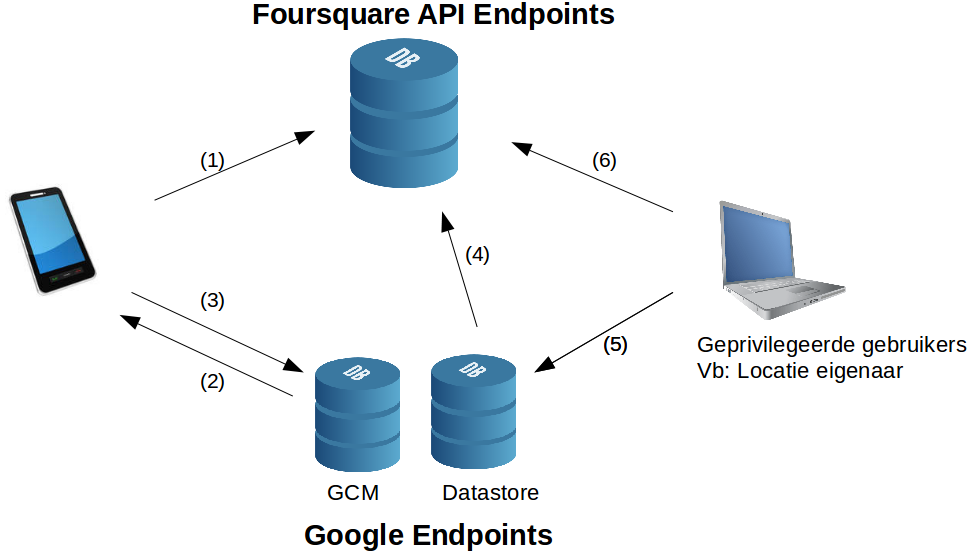
\includegraphics[scale=0.3]{backend_algemene_structuur}
	\caption{Structuur backend}
	\label{fig:algemene structuur backend}

\end{figure}

\section{Backend}

\subsection{Google Cloud Endpoints}
% restricities op aantal request
Google Cloud Endpoints (GCE) is een uitbreiding van Google App Engine (GAE). GAE is een bekend "Platform as a Service" gemaakt om applicaties uit te voeren op de infrastructuur van Google. GCE biedt naast de functionaliteiten beschikbaar in GAE een extra infrastructuur om op een relatief eenvoudige manier een backend API te generen. 
De extra infrastructuur aangeboden door GCE bestaat uit de endpoints. Deze endpoints verzorgen ondermeer de communicatie en authenticatie tussen mobiele gebruikers en de backendserver.
Aangezien de backend API nog steeds gehost wordt door Googles App Engine blijven alle functionaliteiten zoals "Datastore", "Google Cloud Messaging" en "Cron jobs" beschikbaar. Figuur \ref{fig:Architectuur Google Cloud Endpoints} geeft de architectuur van de Enpoint weer~\cite{Google_endpoints}.


Het voornaamste voordeel van het werken met GAE is dat er tijdens ontwikkelfase geen rekening hoeft gehouden te worden met het  beheer en de administratie van de backend infrastructuur. Problemen zoals schaalbaarheid worden via dynamische rekenkracht allocatie opgelost. Daarnaast verzekert de App Engine een permanente beschikbaarheid van de servers worden doorgeschoven.

Desalniettemin brengt het gebruik van GAE meerdere nadelen met zich mee. De voornaamste zijn de restrictie op het aantal lees- en schrijfoperaties per dag, de sterk variërende duratie van lees- en schrijfoperaties en de afhankelijkheid van een externe organistatie. Aangezien elke nieuwe ontwikkelaar \$ 300 cadeau krijgt kon het eerste nadeel opgelost worden door het aantal operaties per dag van 50.000 naar 1.000.000 te verhogen. De reden waarom 1.000.000 operaties per dag noodzakelijk is om Triump draaiende te houden is dat elke entiteit binnen een query als één leesoperatie wordt beschouwd. Hierdoor neemt het aantal leesoperaties bij het uitvoeren van enkele geneste queries zeer snel toe.

\subsubsection{Datastore}

Triump maakt gebruik van App Engine Datastore als backend databank.

GAE Datastore verschillend van traditionele relationele databases door zijn specifieke architectuur. De database is namelijk zo ontworpen dat het automatisch meeschaalt met de toenmende hoeveelheid opgeslagen data. Een tweede verschil met relationele databanken is dat GAE Datastore schemaloos is. Hiermee wordt bedoeld dat objeten van een eenzelfde type verschillende eigenschappen kunnen hebben en dat eenzelfde eigenschap verschillende types kan hebben. 

Objecten in de database worden entiteiten genoemd. Een entiteit heeft meerdere eigenschappen, elk van deze eigenschappen kan één of meerdere waarden hebben. 

Aangezien de database schemaloos is en bijgevolg bijvoorbeeld geen types zal controleren of niet zal aangeven indien een vreemde sleutel niet bestaat ligt de verantwoordelijkheid van het correct houden van de database volledig bij de ontwikkelaar. Tijdens de ontwikkeling werd dit gezien als het grootste nadeel van de Datastore.

\subsubsection{Eigen ontworpen Backend API}

\begin{figure}[H]
	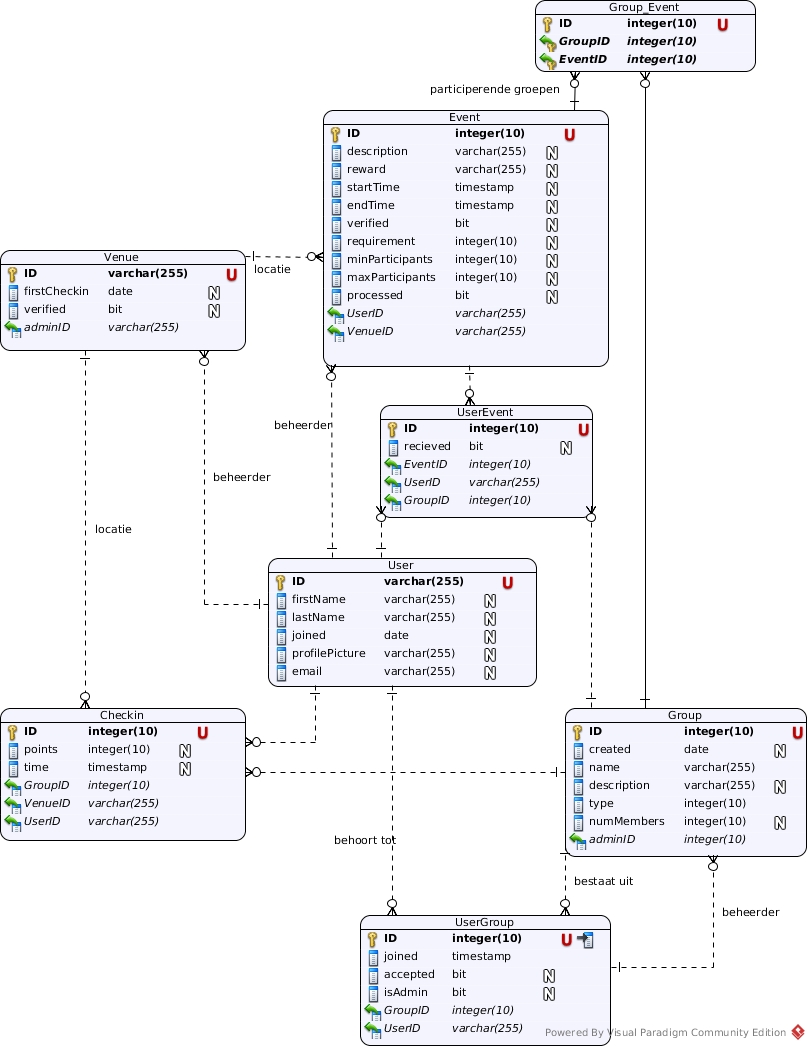
\includegraphics[scale=0.45]{backend_EER}
	\caption{Entity Relation diagram van de backend}
	\label{fig:Backend ER}
\end{figure}

\subsubsection{Google Cloud messaging}
% Notificaties

\subsubsection{Cron jobs}
% Servlet etc...
\subsection{Ontwerpkeuzes}
% EER + verklaring
% Waarom welke data



\subsection{Foursquare API}

%Korte inleiding gebruik API
Zoals reeds eerder aangehaald maakt Triump gebruikt van locaties, deze locaties worden bekomen via de Foursquare application programming interface (API). De Foursquare API geeft de mogelijkheid aan ontwikkelaars om de enorme gebruiker gegenereerde database van Foursquare te raadplegen. Naast locatie gegevens kan er ook informatie van gebruikers zoals namen geboortedata en profielfoto's opgevraagd worden. 

% Overzicht voor en nadelen gebruik API
Het werken met de API brengt echter wel enkele nadelen met zich mee.
Allereerst wordt Triump hierdoor afhankelijk van een externe organisatie. Indien Foursquare beslist zijn open database te sluiten moet het ontwerp van Triump volledig herzien worden. Daarnaast wordt van commerciële applicaties verwacht dat ze reclame maken voor Foursquare door bijvoorbeeld het Foursquare logo op op te nemen in de layout.  Een tweede nadeel is dat de dataopslag verdeeld wordt over twee databases. Enerzijds de Google Cloud Datastore waar de data over groepen en checkins worden bijgehouden en anderzijds de Foursquare Datastore waar de locatie en gebruikergegevens zijn opgeslaan. Een laatste nadeel is dat locaties verplicht geregisteerd moeten zijn bij Foursquare teneinde zichtbaar te zijn op Triump. 

Indien locaties intern zouden aangemaakt en opgeslaan worden zouden de eerste twee nadelen verholpen zijn. 
Deze voor de hand liggende oplossing wordt echter niet toegepast aangezien dit zou impliceren dat Triump vanaf nul zijn locatiedatabase zou moeten vullen. Hierdoor zouden gebruikers ontmoedigd worden Triump boven Foursquare te kiezen. Daarnaast biedt Triump de optie een checkin door te propageren naar Foursquare waardoor we de functionaliteiten ervan uitbreiden. 

Het laatste probleem wordt opgelost door het voorzien van een webinterface. Deze interface voorziet de mogelijkheid aan eigenaars van locaties om de nodige informatie omtrent hun café, zaak of restaurant zichtbaar te maken op Triump. Meer uitleg over de website volgt hieronder.

Er dient opgemerkt te worden dat Google met 'Google Places' gelijkaardige diensten biedt. Gebruik van deze API heeft dezelfde voor- en nadelen als de Foursquare API maar met het bijkomend beperking dat het aantal geregistreerde locaties veel kleiner is.


%werking API
Het mechanisme gebruik in de Foursquare API is zeer vanzelfsprekend. Alle gegevens, opgeslaan in de database, corresponeren met een RESTf URL \cite{FS_API_website}. De frontend applicatie dient een connectie over HTTPS te starten met een Foursquare API Endpoint via de gewenste Uniform Resource Locator (URL). Vervolgens zal de API Endpoint de gevraagde informatie in Javascript Object Notation (JSON) formaat terugzenden. JSON is een gestandaardiseerd gegevensformaat. JSON maakt gebruik van voor de mens leesbare tekst in de vorm van data-objecten die bestaan uit een of meer attributen met bijbehorende waarde. Het wordt hoofdzakelijk gebruikt voor uitwisseling van data tussen server en webapplicatie, als een alternatief voor xml. Het voordeel van JSON is de platformonafhankelijkheid \cite{JSON_def}. In listing ~\ref{lst:vb_foursquare_api} wordt een voorbeeld uitgewerkt waarbij de applicatie vanop de smartphone de informatie van een bepaalde locatie opvraagd.


\begin{lstlisting}[caption={Voorbeeld: werking Foursquare API},label=lst:vb_foursquare_api]

HTTPS connectie naar URL:
https://api.foursquare.com/v2/venues/4d972f73af3d236ad0561cc7?
	oauth_token=OMUUXC42I4GCMV3G21&v=20150101&m=foursquare

Antwoord:
"venue":
	{
	"id":"4d972f73af3d236ad0561cc7",
	"name":"POM D' API BRUXELLES",
	"contact":{},
	"location":
		{
		"address":"Koninginnegallerij",
		"lat":50.0,"lng":4.0,
		"postalCode":"1000",
		"city":"Brussels",
		"state":"Bruxelles-Capitale",
		"country":"Belgium",
		"formattedAddress":
		["Koninginnegallerij","1000 Brussels"]
		}
	}
\end{lstlisting}
 


\section{Frontend}
\subsection{Android applicatie}
\subsubsection{Waarom Android}
% Keuze android boven iOS
% 
\subsubsection{Ontwikkelomgeving: Android Studio}
% vergelijking vs Eclipse
\subsubsection{Inloggen via Foursquare}

\subsubsection{Ontwerpkeuzes}
% Recycler view, nieuwste trends
% material design: welke lib. dat we gebruikt hebben
% Loadermechanismen
% Lokale SQLite DB
% Cardmechanisme

\subsection{Webinterface}
\subsubsection{Doel}
% De Waarom Vraag
Voor een aantal taken is een smartphone niet helemaal geschikt. Deze heeft een klein scherm en de touchbediening is niet altijd handig. Zulke taken zijn het beheren van groepen en het aanmaken van promoties.
Deze taken moeten redelijk vaak gebeuren en gebeuren gemakkelijker op een groter scherm. Specifieke gebruikers, zoals uitbaters van locaties die een promotie willen opzetten om zo klanten te lokken, zullen deze taken willen uitvoeren. Daarom is Triump uitgebreid met een webinterface.
Onze site zal tevens dienst doen als infopunt voor huidige en toekomstige gebruikers. Op de site staat informatie over wat het doel is van Triump en waarom gebruikers
Op onze website kunnen gebruikers net als in de android-applicatie inloggen met Foursquare. Het is de bedoeling dat het registereren van een Foursquare-locatie steeds via de website gebeurd, net als het aanmaken van promoties door een eigenaar van een registreerde locatie.
\subsubsection{Django-framework}
Bij het maken van een website kan men verschillende keuzes maken.
Eerst en vooral is er de keuze of er gebruik wordt gemaakt van een bestaand framework, zoals Ruby on Rails, ASP.NET en Django, of dat men zelf met bijvoorbeeld PHP de nodige functionaliteit implementeert.
Omdat de webinterface slechts extra functionaliteit mogelijk maakt en dus niet het grootste deel van ons project is, werd besloten om deze voorlopig niet te uitgebreid te maken.
Het helemaal zelf opbouwen van de site is daarom een slecht idee: bestaande frameworks bieden ruim voldoende functionaliteit aan om onze website te maken. De frameworks zijn daarboven reeds geoptimaliseerd en bevatten functies zoals een standaardmanier om gebruikers veilig in te loggen. Het inloggen helemaal zelf implementeren daarintegen zou veel tijd en werk vragen, terwijl de kwaliteit naar alle waarschijnlijkheid beneden die van bestaande oplossingen zou liggen. 
Daarnaast moet men nog kiezen om ofwel de site bij een hosting-dienst te plaatsen, of zelfs de hosting te voorzien. De hosting zelf voorzien brengt vele moeilijkheden met zich mee: liefst wordt er gewerkt met een vast IP-adres, maar providers kennen aan gewone klanten slechts een tijdelijk IP-adres toe. Daarboven dient men dan ook de DNS-servers (minmaal 2) zelf te verzorgen.
De andere oplossing, gebruik maken van een hosting-dienst, is veel eenvoudiger. Voor een vast bedrag, per maand of jaar, wordt de website geplaatst op de servers van de hosting-dienst. Deze neemt extra moeilijkheden, zoals het instellen en onderhouden van DNS-servers op zich.
Het databasemanagment systeem moet ook nog worden gekozen indien dit van toepassing is. Hier was dit het geval: op de site worden gebruikers aangemaakt waarbij bepaalde informatie wordt opgeslaan, zoals hun Foursquare-identiteit, zodat de gebruiker maar 1 keer met Foursquare moet inloggen.
Kozen voor Django: draait op python: eenvoudig, maar krachtig
Webhosting: http://djangoeurope.com/ gespecialiseerd in django projecten, bieden all-in-one pakket aan voor een goede prijs
PostgreSql: databank waar we mee hebben gewerkt tijdens het vak "Databanken"
